\documentclass[
    12pt,           % tamanho da fonte do texto
    oneside,        % impressão em um lado da folha
    a4paper,        % tamanho do papel
    chapter=TITLE,  % títulos de capítulos em caixa alta
    english,        % idioma adicional para pacotes internos
    brazil          % idioma principal do documento
]{abntex2}

\usepackage[utf8]{inputenc}      % codificação de entrada UTF-8
\usepackage[T1]{fontenc}         % codificação de fonte
\usepackage{indentfirst}         % recuo na primeira linha dos parágrafos
\usepackage{graphicx}            % inserção de imagens (uso futuro)
\usepackage{microtype}           % melhorias tipográficas sutis
\usepackage{newtxtext}           % fonte Times New Roman
\usepackage{pifont}              % ícones para tabela (check e cross)
\usepackage{xcolor}              % suporte a cores
\usepackage{longtable}           % tabelas que quebram entre páginas (requisitos)

\usepackage[alf]{abntex2cite}

% MARGENS superior 3 cm | esquerda 3 cm | inferior 2 cm | direita 2 cm
\usepackage[
    top=3cm,
    left=3cm,
    bottom=2cm,
    right=2cm
]{geometry}


% ESPAÇAMENTO E FORMATAÇÃO DE PARÁGRAFO
\OnehalfSpacing                  % espaçamento 1,5 entre linhas
\setlength{\parindent}{1.25cm}   % recuo de parágrafo
\setlength{\parskip}{0pt}        % sem espaçamento extra entre parágrafos


% FONTES E TAMANHOS DOS TÍTULOS (CAPÍTULOS, SEÇÕES E SUBSEÇÕES)
\renewcommand{\ABNTEXchapterfontsize}{\fontsize{12}{14}\selectfont}
\renewcommand{\ABNTEXsectionfontsize}{\fontsize{12}{14}\selectfont}
\renewcommand{\ABNTEXsubsectionfontsize}{\fontsize{12}{14}\selectfont}
\renewcommand{\ABNTEXsubsubsectionfontsize}{\fontsize{12}{14}\selectfont}

\renewcommand{\ABNTEXchapterfont}{\rmfamily\bfseries}
\renewcommand{\ABNTEXsectionfont}{\rmfamily\bfseries}
\renewcommand{\ABNTEXsubsectionfont}{\rmfamily\bfseries}
\renewcommand{\ABNTEXsubsubsectionfont}{\rmfamily\itshape}

\setlength{\beforechapskip}{0pt}
\setlength{\afterchapskip}{\baselineskip}


% TABELAS
\newcommand{\cmark}{\textcolor{green!60!black}{\ding{51}}}  % Símbolo de visto (verde)
\newcommand{\xmark}{\textcolor{red}{\textbf{X}}}            % Símbolo de X (vermelho)


% INFORMAÇÕES DO DOCUMENTO
\titulo{CLASSIFICAÇÃO INTELIGENTE DE CONTEÚDO WEB PARA CONTROLE DE ACESSO EM NAVEGADORES}
\autor{%
    Eduarda Luiza Pinheiro Nepomuceno \\
    Jean Yuki Kimura \\
    Jhenifer Laís Barbosa \\
    João Pedro Duarte Giatti
}

% CONFIGURAÇÕES DE PDF (metadados)
\makeatletter
\hypersetup{
    pdftitle={\@title},
    pdfauthor={\@author},
    pdfsubject={Engenharia de Software},
    pdfkeywords={Inteligência Artificial. Segurança digital. Controle parental. Classificação de conteúdo. Navegadores. Processamento de linguagem natural},
    colorlinks=false,
    pdfborder={0 0 0}
}
\makeatother

\begin{document}

% ------------------------------------------------------------
% CAPA
% ------------------------------------------------------------
\begin{capa}
    \center

    {\bfseries\fontsize{12}{14}\selectfont PONTIFÍCIA UNIVERSIDADE CATÓLICA DE CAMPINAS}\par
    {\bfseries\fontsize{12}{14}\selectfont ENGENHARIA DE SOFTWARE}\par
    {\bfseries\fontsize{12}{14}\selectfont 12563 - PROJETO INTEGRADOR VI - ENGENHARIA DE SOFTWARE}\par

    \vfill

    {\bfseries\fontsize{12}{14}\selectfont
        \imprimirtitulo\par}

    \vfill

    {\bfseries\fontsize{12}{16}\selectfont
        24002529 EDUARDA LUIZA PINHEIRO NEPOMUCENO\par
        24008214 JEAN YUKI KIMURA\par
        24014979 JHENIFER LAÍS BARBOSA\par
        24019083 JOÃO PEDRO DUARTE GIATTI\par
    }

    \vfill

    {\bfseries\fontsize{12}{14}\selectfont
        ORIENTADORA: SÍLVIA CRISTINA DE MATOS SOARES\par
    }

    \vfill

    {\bfseries\fontsize{12}{14}\selectfont
        CAMPINAS\par
        2º SEMESTRE DE 2026\par
    }
\end{capa}

% ------------------------------------------------------------
% RESUMO
% ------------------------------------------------------------
\begin{resumo}
    \SingleSpacing

    O acesso frequente de crianças e adolescentes à internet por meio de
    computadores e navegadores torna relevante o desenvolvimento de mecanismos
    capazes de identificar e reduzir a exposição a conteúdos potencialmente
    inadequados. Neste semestre, este projeto propõe o desenvolvimento e a
    validação de um sistema executado em nível de máquina, associado ao uso de
    um navegador, capaz de obter o conteúdo textual e as imagens das páginas
    acessadas e submetê-los a modelos de inteligência artificial para
    classificação automática, seguindo dois caminhos técnicos complementares:
    processamento de linguagem natural, para o conteúdo textual, e visão
    computacional, para o conteúdo visual. Os modelos serão treinados ou
    ajustados (\textit{fine-tuned}) pela equipe para classificar conteúdos em
    categorias previamente definidas, permitindo que um mecanismo de políticas
    consolide as classificações e determine se determinado conteúdo deve ser
    permitido ou bloqueado. O sistema também deverá registrar informações
    relevantes sobre as classificações e ações realizadas, de modo a
    possibilitar a apresentação de estatísticas e histórico por meio de uma
    interface de acompanhamento. O escopo deste semestre está concentrado na
    construção e validação dos motores de classificação textual e de imagem e
    de sua aplicação em nível de máquina, não contemplando ainda a
    implementação de um \textit{gateway} de rede ou a identificação de
    usuários por endereço IP.
    Como evolução planejada para os semestres seguintes, o núcleo desenvolvido
    será integrado a uma infraestrutura baseada em Raspberry Pi, permitindo a
    aplicação centralizada de políticas a diferentes dispositivos de uma rede
    doméstica e, posteriormente, a expansão da solução para outros cenários de
    controle e segurança digital. Espera-se, ao final deste semestre, obter um
    protótipo funcional e mensurável, com suas métricas de desempenho e
    limitações técnicas devidamente documentadas.

    \vspace{\onelineskip}
    \noindent

    \textbf{Palavras-chave}: Inteligência Artificial. Segurança digital. Controle parental. Classificação de conteúdo. Navegadores. Processamento de linguagem natural. Visão computacional.
\end{resumo}

% ------------------------------------------------------------
% SUMÁRIO
% ------------------------------------------------------------
\pdfbookmark[0]{\contentsname}{sumario}
\tableofcontents*
\cleardoublepage
\textual
\pagestyle{simple}

% ------------------------------------------------------------
% 1 INTRODUÇÃO
% ------------------------------------------------------------
\chapter{Introdução}

O acesso à internet por crianças e adolescentes ocorre, cada vez mais, por meio
de navegadores instalados em computadores e outros dispositivos de uso pessoal.
Embora a internet ofereça importantes recursos para educação, comunicação e
entretenimento, a variedade e a velocidade de publicação de conteúdos também
dificultam a identificação manual de materiais potencialmente inadequados.

As soluções tradicionais de controle de acesso frequentemente dependem de
listas de bloqueio, categorias previamente cadastradas ou configurações
realizadas individualmente em cada dispositivo. Essas abordagens podem
apresentar limitações diante de páginas novas, conteúdos dinâmicos e situações
em que um mesmo domínio disponibiliza materiais de naturezas distintas. Nesse
contexto, técnicas de inteligência artificial podem ser utilizadas para analisar
o conteúdo textual e o conteúdo visual (imagens) de uma página e estimar a
quais categorias de conteúdo ela pertence, oferecendo uma camada adicional de
decisão.

Este projeto tem como foco o desenvolvimento, neste semestre, de um sistema em
nível de máquina voltado à análise do conteúdo textual e do conteúdo visual
(imagens) de páginas acessadas por meio de um navegador. A proposta consiste
em obter o conteúdo textual e as imagens disponíveis durante a navegação,
submetê-los a modelos de inteligência artificial treinados ou ajustados pela
equipe — um voltado ao texto e outro às imagens — e produzir classificações
associadas a categorias previamente definidas. A partir dessas classificações,
um mecanismo de políticas poderá determinar se o conteúdo deve ser permitido
ou bloqueado de acordo com as regras estabelecidas para o cenário de uso.

A arquitetura proposta separa a responsabilidade de classificação da
responsabilidade de decisão. Os modelos de inteligência artificial deverão
responder à pergunta ``que tipo de conteúdo está presente?'' — cada um a
partir de sua modalidade (texto ou imagem) —, enquanto o mecanismo de
políticas deverá responder ``esse conteúdo é permitido para este contexto?'',
consolidando as classificações recebidas. Essa separação permite que as
mesmas classificações sejam utilizadas por diferentes conjuntos de regras e
possibilita a evolução posterior da solução para outros ambientes.

Para este semestre, o projeto seguirá dois caminhos técnicos complementares
de inteligência artificial: a análise textual, com a utilização de técnicas
de processamento de linguagem natural (PLN), e a análise visual, com a
utilização de técnicas de visão computacional aplicadas às imagens presentes
nas páginas. Os dois modelos serão treinados ou ajustados
(\textit{fine-tuned}) a partir de dados apropriados para as categorias
definidas pela equipe. Suas avaliações serão realizadas por meio de métricas
como precisão, \textit{recall}, F1-\textit{score}, taxas de falsos positivos
e falsos negativos e tempo de classificação, permitindo medir não apenas a
capacidade de classificação de cada modelo, mas também a viabilidade de sua
utilização conjunta em um cenário de navegação.

O projeto também poderá disponibilizar uma interface de acompanhamento, na
qual informações como classificações realizadas (textuais e de imagem),
conteúdos bloqueados e estatísticas de uso possam ser consultadas. Essa
interface tem caráter de apoio ao acompanhamento e à avaliação do protótipo,
não constituindo, neste semestre, um painel de administração de uma rede
doméstica.

É importante delimitar o escopo desta etapa. O sistema desenvolvido terá como
escopo: (i) um mecanismo em nível de máquina associado à navegação por
navegador; (ii) a obtenção e o processamento do conteúdo textual e das
imagens das páginas acessadas; (iii) um modelo de processamento de linguagem
natural e um modelo de visão computacional, treinados ou ajustados pela
equipe, para classificação do conteúdo textual e visual, respectivamente, em
categorias definidas; (iv) um mecanismo de aplicação de políticas capaz de
consolidar as classificações textual e de imagem e de permitir ou bloquear
conteúdos de acordo com elas; e (v) o registro e a apresentação de
informações necessárias para testes, validação e acompanhamento do sistema.

Não fazem parte do escopo deste semestre: a implementação do Raspberry Pi como
\textit{gateway} de rede; a identificação de usuários ou dispositivos por
endereço IP em nível de rede; a aplicação centralizada de políticas para
múltiplos dispositivos; e a análise do tráfego criptografado ponto a ponto.
Também não se pretende garantir o bloqueio absoluto de todo conteúdo
inadequado presente na internet. A solução será apresentada como um mecanismo
de redução da exposição a conteúdos potencialmente inadequados, considerando
as limitações inerentes à obtenção de conteúdo textual e de imagens, ao
funcionamento dos navegadores, ao uso de HTTPS e à natureza dinâmica da web.

\section*{Evolução planejada do projeto}

A solução desenvolvida neste semestre constitui o núcleo inicial de uma
proposta de maior abrangência para os semestres seguintes. Como evolução
planejada, os motores de classificação textual e de imagem deverão ser
integrados a uma infraestrutura baseada em Raspberry Pi, que atuará como
ponto central de controle em uma rede doméstica. Nessa etapa futura, será
possível associar dispositivos e,
posteriormente, usuários ou perfis a políticas específicas e aplicar as
decisões de acesso de maneira centralizada.

Em uma etapa posterior, a solução poderá incorporar um painel administrativo
voltado a responsáveis, permitindo configurar perfis, políticas e horários,
além de acompanhar estatísticas e tentativas de acesso bloqueadas. A
arquitetura também poderá ser expandida para cenários além do controle
parental, como ambientes educacionais e empresariais, nos quais a classificação
inteligente de conteúdo possa auxiliar na redução de riscos de segurança
digital.

\section*{Círculo Dourado}

Para explicitar o propósito do projeto, aplica-se o modelo do Círculo Dourado
(\textit{Golden Circle}), de Simon Sinek, estruturado em três camadas:
\textit{Why} (por quê), \textit{How} (como) e \textit{What} (o quê).

\begin{alineas}
    \item \textbf{Why (Por quê):} Acreditamos que responsáveis devem possuir meios acessíveis de reduzir a exposição de crianças e adolescentes a conteúdos potencialmente inadequados na internet, sem depender exclusivamente de listas estáticas de bloqueio ou de configurações técnicas complexas.
    \item \textbf{How (Como):} Neste semestre, isso será investigado por meio de um sistema em nível de máquina capaz de analisar o conteúdo textual e o conteúdo visual (imagens) de páginas acessadas no navegador, utilizando um modelo de processamento de linguagem natural e um modelo de visão computacional, treinados ou ajustados pela equipe, para classificá-los segundo categorias previamente definidas. As classificações serão então consolidadas e utilizadas por um mecanismo de políticas para determinar a ação de acesso.
    \item \textbf{What (O quê):} O resultado deste semestre será um protótipo funcional de classificação e controle de conteúdo textual e visual em nível de máquina, acompanhado de métricas de avaliação de cada modalidade e, quando aplicável, uma interface para acompanhamento das classificações e bloqueios. Nos semestres seguintes, esse núcleo será integrado a uma infraestrutura de rede baseada em Raspberry Pi, com o objetivo de evoluir para uma solução centralizada de controle de acesso.
\end{alineas}

\vspace{0.5cm}

\begin{figure}[htbp]
    \centering
    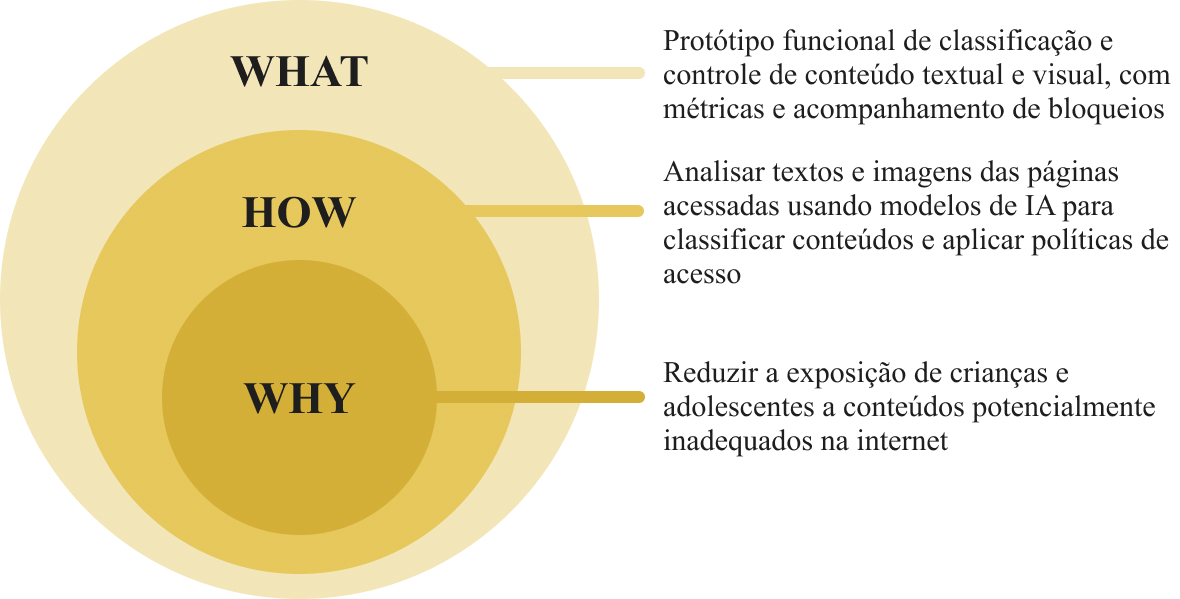
\includegraphics[width=0.95\textwidth]{circulo-dourado.jpg}
    \caption{Círculo Dourado}
    \label{fig:circulo-dourado}
\end{figure}

% ------------------------------------------------------------
% 2 OBJETIVOS
% ------------------------------------------------------------
\chapter{Objetivos}

\section{Objetivo Geral}

Desenvolver e validar um protótipo em nível de máquina capaz de analisar o
conteúdo textual e o conteúdo visual (imagens) de páginas acessadas por meio
de um navegador, utilizando um modelo de processamento de linguagem natural e
um modelo de visão computacional, treinados ou ajustados (\textit{fine-tuned})
pela equipe, para classificar conteúdos em categorias previamente definidas e
aplicar políticas de permissão ou bloqueio a partir da consolidação dessas
classificações.

\section{Objetivos Específicos}

\begin{alineas}
    \item Pesquisar e selecionar técnicas de processamento de linguagem natural e de visão computacional, bem como modelos de inteligência artificial adequados à classificação de conteúdo textual e visual de páginas web, considerando as restrições de execução e resposta esperadas para um sistema em nível de máquina;
    \item Construir, preparar e documentar bases de dados (textual e de imagens) para treinamento, validação e teste dos modelos, definindo categorias de conteúdo e procedimentos de pré-processamento compatíveis com cada modalidade;
    \item Treinar ou ajustar (\textit{fine-tune}) um modelo de processamento de linguagem natural e um modelo de visão computacional para classificar, respectivamente, o conteúdo textual e as imagens das páginas nas categorias definidas, buscando reduzir a dependência de listas estáticas de sites;
    \item Desenvolver o mecanismo em nível de máquina responsável por obter o conteúdo textual e as imagens das páginas acessadas pelo navegador e encaminhá-los aos respectivos classificadores, respeitando as limitações técnicas impostas pelo funcionamento da web e pelo uso de conexões criptografadas;
    \item Desenvolver um mecanismo de políticas que utilize e consolide as classificações textual e de imagem produzidas pela inteligência artificial para determinar se determinado conteúdo deve ser permitido ou bloqueado, mantendo separadas as responsabilidades de classificação e decisão;
    \item Implementar, quando aplicável ao protótipo, uma interface de acompanhamento das classificações e ações realizadas, permitindo visualizar informações como conteúdos analisados (por modalidade), bloqueios e estatísticas de uso;
    \item Avaliar o desempenho dos classificadores textual e de imagem por meio de métricas como precisão, \textit{recall}, F1-\textit{score}, taxa de falsos positivos, taxa de falsos negativos e tempo de classificação, analisando os resultados obtidos, isoladamente e em conjunto, e suas limitações;
    \item Realizar testes do sistema em diferentes situações de navegação, verificando a integração entre obtenção do conteúdo textual e visual, classificação, consolidação das classificações, aplicação das políticas e registro dos resultados;
    \item Identificar e documentar as limitações técnicas, éticas e de privacidade da solução, especialmente aquelas relacionadas ao monitoramento de navegação, à obtenção de conteúdo textual e de imagens, à classificação automatizada e ao uso de dados de navegação;
    \item Estabelecer uma base arquitetural que permita, nos semestres seguintes, a integração dos motores de classificação textual e de imagem a uma infraestrutura de rede baseada em Raspberry Pi e a evolução da solução para aplicação centralizada de políticas em múltiplos dispositivos.
\end{alineas}

% ------------------------------------------------------------
% 3 Representantes da Comunidade Externa
% ------------------------------------------------------------
\chapter{Representantes da Comunidade Externa}

Caracterizar a extensão (62 horas de extensão) - são as pessoas que participarão da
definição, das entrevistas, da definição dos requisitos, da validação dos protótipos e da
validação final do projeto).

Nome, contato (e-mail) e cargo do profissional/pessoa e o nome e CNPJ da organização
onde ele(a) atua (2 a 5 profissionais).

% ------------------------------------------------------------
% 4 Fundamentação Teórica
% ------------------------------------------------------------
\chapter{Fundamentação Teórica}

Apresentar os conceitos teóricos relacionados à tecnologia atual e Engenharia de Software
que embasam o projeto.

Incluir a definição das técnicas/ferramentas/algoritmos etc. das tecnologias atuais
utilizadas.

% ------------------------------------------------------------
% 5 Levantamento e Análise de Requisitos
% ------------------------------------------------------------

% --- Macros do template de requisitos funcionais (sem pacotes extras) ---
\newenvironment{dadoslista}{%
  \begin{itemize}%
  \setlength{\leftmargin}{1.1em}\setlength{\labelwidth}{0.7em}%
  \setlength{\labelsep}{0.4em}\setlength{\itemsep}{0pt}%
  \setlength{\parsep}{0pt}\setlength{\topsep}{0pt}\setlength{\partopsep}{0pt}}%
  {\end{itemize}}

\newcommand{\reqfunc}[5]{%
  \par\medskip\noindent
  \begin{tabular}{|p{3.3cm}|p{10.4cm}|}
  \hline
  \textbf{Identificador} & \textbf{#1} \\ \hline
  \textbf{Nome} & #2 \\ \hline
  \textbf{Descrição Geral} & #3 \\ \hline
  \textbf{Atores} & #4 \\ \hline
  \textbf{Informações / Dados} & #5 \\ \hline
  \end{tabular}
  \par\medskip}

\chapter{Levantamento e Análise de Requisitos}

\section{Requisitos Funcionais}

Os requisitos funcionais são descritos no formato de histórias de usuário da
metodologia ágil (\textit{``Eu, enquanto <quem>, quero <o quê>, para <por quê>''}).
O Quadro~\ref{tab:requisitos-funcionais} resume os requisitos e suas prioridades;
o detalhamento de cada um segue logo após.

\begin{longtable}{|p{1.6cm}|p{9.8cm}|p{2.3cm}|}
\hline
\textbf{Código} & \textbf{Nome} & \textbf{Prioridade} \\ \hline
\endfirsthead
\hline
\textbf{Código} & \textbf{Nome} & \textbf{Prioridade} \\ \hline
\endhead

RF001 & Captura de conteúdo das páginas & Essencial \\ \hline
RF002 & Pré-processamento do conteúdo textual & Essencial \\ \hline
RF003 & Classificação textual (PLN) & Essencial \\ \hline
RF004 & Nível de confiança da classificação textual & Essencial \\ \hline
RF005 & Pré-processamento de imagens & Essencial \\ \hline
RF006 & Classificação de imagens (visão computacional) & Essencial \\ \hline
RF007 & Nível de confiança da classificação de imagem & Essencial \\ \hline
RF008 & Consolidação das classificações de texto e imagem & Essencial \\ \hline
RF009 & Aplicação do mecanismo de políticas & Essencial \\ \hline
RF010 & Configuração de regras de política por categoria & Importante \\ \hline
RF011 & Bloqueio de acesso com mensagem informativa & Essencial \\ \hline
RF012 & Registro (log) das classificações & Essencial \\ \hline
RF013 & Consulta do histórico de classificações e bloqueios & Importante \\ \hline
RF014 & Estatísticas de uso & Importante \\ \hline
RF015 & Início e pausa do monitoramento & Importante \\ \hline

\caption{Requisitos Funcionais}
\label{tab:requisitos-funcionais}
\end{longtable}

\reqfunc{RF001}
{Captura de conteúdo das páginas}
{Eu, enquanto responsável pelo monitoramento, quero que o sistema obtenha o conteúdo textual e as imagens das páginas acessadas durante a navegação, para que esse conteúdo possa ser analisado e classificado.}
{\begin{dadoslista}
\item Usuário monitorado (navega pelas páginas)
\item Extensão do navegador (coleta o conteúdo)
\end{dadoslista}}
{\begin{dadoslista}
\item \textbf{Entrada:} URL/domínio e DOM da página acessada
\item \textbf{Saída:} texto bruto da página, lista de imagens (origem e dimensões) e data/hora da captura
\end{dadoslista}}

\reqfunc{RF002}
{Pré-processamento do conteúdo textual}
{Eu, enquanto responsável pelo monitoramento, quero que o texto obtido seja limpo e normalizado antes da classificação, para que o classificador receba conteúdo livre de ruído e produza resultados mais precisos.}
{\begin{dadoslista}
\item Módulo de pré-processamento textual (sistema)
\end{dadoslista}}
{\begin{dadoslista}
\item \textbf{Entrada:} texto bruto (com marcações HTML, menus, rodapés e \textit{scripts})
\item \textbf{Saída:} texto limpo e normalizado
\item \textbf{Parâmetros:} tamanho mínimo e máximo de texto (ex.: mínimo de 50 palavras; máximo de 512 \textit{tokens})
\end{dadoslista}}

\reqfunc{RF003}
{Classificação textual (PLN)}
{Eu, enquanto responsável pelo monitoramento, quero que o texto pré-processado seja classificado por um modelo de PLN em categorias previamente definidas, para identificar conteúdo textual potencialmente inadequado.}
{\begin{dadoslista}
\item Módulo de PLN (sistema)
\end{dadoslista}}
{\begin{dadoslista}
\item \textbf{Entrada:} texto pré-processado
\item \textbf{Saída:} categoria textual atribuída e versão do modelo utilizada
\item \textbf{Categorias:} definidas pela equipe (ex.: seguro, sexual, violência, drogas, jogos de azar, discurso de ódio)
\end{dadoslista}}

\reqfunc{RF004}
{Nível de confiança da classificação textual}
{Eu, enquanto responsável pelo monitoramento, quero que cada classificação textual tenha um nível de confiança associado, para que a decisão do sistema leve em conta a certeza do modelo de PLN.}
{\begin{dadoslista}
\item Módulo de PLN (sistema)
\item Mecanismo de políticas (consome o \textit{score})
\end{dadoslista}}
{\begin{dadoslista}
\item \textbf{Entrada:} saída do modelo de PLN
\item \textbf{Saída:} \textit{score} de confiança no intervalo [0, 1] associado à categoria atribuída
\end{dadoslista}}

\reqfunc{RF005}
{Pré-processamento de imagens}
{Eu, enquanto responsável pelo monitoramento, quero que as imagens obtidas sejam redimensionadas, normalizadas e filtradas antes da classificação, para que apenas imagens relevantes sejam analisadas e o tempo de resposta seja adequado.}
{\begin{dadoslista}
\item Módulo de pré-processamento de imagens (sistema)
\end{dadoslista}}
{\begin{dadoslista}
\item \textbf{Entrada:} imagens brutas da página
\item \textbf{Saída:} imagens redimensionadas e normalizadas no formato de entrada do modelo
\item \textbf{Critérios de descarte:} ícones e imagens de interface; dimensão mínima (ex.: 100$\times$100 px); limite de imagens por página (ex.: as 10 a 20 maiores)
\item \textbf{Parâmetro:} tamanho de entrada do modelo (ex.: 224$\times$224 px)
\end{dadoslista}}

\reqfunc{RF006}
{Classificação de imagens (visão computacional)}
{Eu, enquanto responsável pelo monitoramento, quero que as imagens pré-processadas sejam classificadas por um modelo de visão computacional em categorias previamente definidas, para identificar conteúdo visual potencialmente inadequado.}
{\begin{dadoslista}
\item Módulo de visão computacional (sistema)
\end{dadoslista}}
{\begin{dadoslista}
\item \textbf{Entrada:} imagens pré-processadas
\item \textbf{Saída:} categoria visual atribuída a cada imagem e versão do modelo utilizada
\item \textbf{Categorias:} definidas pela equipe, com mapeamento para as categorias textuais
\end{dadoslista}}

\reqfunc{RF007}
{Nível de confiança da classificação de imagem}
{Eu, enquanto responsável pelo monitoramento, quero que cada classificação de imagem tenha um nível de confiança associado, para que a decisão do sistema leve em conta a certeza do modelo de visão computacional.}
{\begin{dadoslista}
\item Módulo de visão computacional (sistema)
\item Mecanismo de políticas (consome o \textit{score})
\end{dadoslista}}
{\begin{dadoslista}
\item \textbf{Entrada:} saída do modelo de visão computacional
\item \textbf{Saída:} \textit{score} de confiança no intervalo [0, 1] associado à categoria atribuída
\end{dadoslista}}

\reqfunc{RF008}
{Consolidação das classificações de texto e imagem}
{Eu, enquanto responsável pelo monitoramento, quero que as classificações textual e de imagem de uma mesma página sejam consolidadas em uma decisão única, com critério de precedência para os casos de divergência, para que o mecanismo de políticas receba um resultado coerente.}
{\begin{dadoslista}
\item Módulo de consolidação (sistema)
\end{dadoslista}}
{\begin{dadoslista}
\item \textbf{Entrada:} categoria e \textit{score} textuais; categoria(s) e \textit{score}(s) de imagem
\item \textbf{Regra de precedência:} em caso de divergência, prevalece a classificação associada à ação mais restritiva da política (bloquear $>$ alertar $>$ permitir)
\item \textbf{Saída:} decisão consolidada (categoria, \textit{score} e modalidade de origem)
\end{dadoslista}}

\reqfunc{RF009}
{Aplicação do mecanismo de políticas}
{Eu, enquanto responsável pelo monitoramento, quero que um mecanismo de políticas determine, a partir da decisão consolidada, se o conteúdo deve ser permitido, bloqueado ou alertado, para que a navegação do usuário seja controlada de acordo com as regras definidas.}
{\begin{dadoslista}
\item Mecanismo de políticas (sistema)
\item Responsável (define as regras)
\end{dadoslista}}
{\begin{dadoslista}
\item \textbf{Entrada:} decisão consolidada (RF008) e regras por categoria (RF010)
\item \textbf{Parâmetros:} limiares de confiança (ex.: $\geq$ 0,80 bloqueia; entre 0,50 e 0,80 alerta; $<$ 0,50 permite; limiar de bloqueio menor nas categorias sensíveis)
\item \textbf{Saída:} ação a ser tomada (permitir, bloquear ou alertar)
\end{dadoslista}}

\reqfunc{RF010}
{Configuração de regras de política por categoria}
{Eu, enquanto responsável pelo monitoramento, quero configurar a ação (permitir, bloquear ou alertar) para cada categoria de conteúdo, para adequar a proteção ao perfil do usuário monitorado.}
{\begin{dadoslista}
\item Responsável
\end{dadoslista}}
{\begin{dadoslista}
\item \textbf{Entrada:} categoria, ação desejada e, opcionalmente, limiar de confiança
\item \textbf{Saída:} conjunto de regras persistido e aplicado pelo mecanismo de políticas
\end{dadoslista}}

\reqfunc{RF011}
{Bloqueio de acesso com mensagem informativa}
{Eu, enquanto responsável pelo monitoramento, quero que o acesso seja bloqueado e uma mensagem informativa seja exibida ao usuário quando a política determinar o bloqueio, para impedir a exposição ao conteúdo e deixar claro o motivo da restrição.}
{\begin{dadoslista}
\item Usuário monitorado (visualiza a mensagem)
\item Extensão do navegador (executa o bloqueio)
\end{dadoslista}}
{\begin{dadoslista}
\item \textbf{Entrada:} ação ``bloquear'', URL da página e categoria atribuída
\item \textbf{Saída:} página de bloqueio com mensagem informativa
\end{dadoslista}}

\reqfunc{RF012}
{Registro (log) das classificações}
{Eu, enquanto responsável pelo monitoramento, quero que cada classificação realizada seja registrada, para permitir o acompanhamento e a auditoria das decisões do sistema.}
{\begin{dadoslista}
\item Módulo de registro (sistema)
\item Responsável (consulta os registros)
\end{dadoslista}}
{\begin{dadoslista}
\item \textbf{Campos:} URL/domínio, modalidade (texto e/ou imagem), categoria atribuída, nível de confiança, ação tomada, data/hora e versão do modelo
\item \textbf{Observação:} o conteúdo integral (texto e imagens) não deve ser armazenado além do necessário (RNF003)
\end{dadoslista}}

\reqfunc{RF013}
{Consulta do histórico de classificações e bloqueios}
{Eu, enquanto responsável pelo monitoramento, quero consultar o histórico de classificações e bloqueios em uma interface de acompanhamento, para saber quais conteúdos foram analisados e quais ações foram tomadas.}
{\begin{dadoslista}
\item Responsável
\end{dadoslista}}
{\begin{dadoslista}
\item \textbf{Entrada:} filtros opcionais (período, categoria, ação, modalidade, domínio)
\item \textbf{Saída:} lista de registros de classificação conforme os filtros
\end{dadoslista}}

\reqfunc{RF014}
{Estatísticas de uso}
{Eu, enquanto responsável pelo monitoramento, quero visualizar estatísticas de uso na interface de acompanhamento, para entender o padrão de navegação e a atuação do sistema ao longo do tempo.}
{\begin{dadoslista}
\item Responsável
\end{dadoslista}}
{\begin{dadoslista}
\item \textbf{Entrada:} período consultado (ex.: 24 h, 7 dias, 30 dias ou personalizado)
\item \textbf{Saída:} total de páginas analisadas, distribuição por categoria e percentual bloqueado por modalidade
\end{dadoslista}}

\reqfunc{RF015}
{Início e pausa do monitoramento}
{Eu, enquanto responsável pelo monitoramento, quero iniciar ou pausar o monitoramento, para controlar quando a análise da navegação está ativa.}
{\begin{dadoslista}
\item Responsável
\item Usuário monitorado (afetado pelo estado do monitoramento)
\end{dadoslista}}
{\begin{dadoslista}
\item \textbf{Entrada:} comando de iniciar ou pausar e, se aplicável, autenticação do responsável (ex.: PIN)
\item \textbf{Saída:} estado atual (ativo ou pausado) e registro da alteração com data/hora
\end{dadoslista}}

\section{Requisitos Não Funcionais}

Os requisitos não funcionais descrevem atributos de qualidade do sistema,
organizados a partir de categorias inspiradas na norma ISO/IEC~25010.

\begin{longtable}{|p{1.5cm}|p{3.2cm}|p{6.8cm}|p{2.2cm}|}
\hline
\textbf{Código} & \textbf{Categoria} & \textbf{Descrição} & \textbf{Prioridade} \\ \hline
\endfirsthead
\hline
\textbf{Código} & \textbf{Categoria} & \textbf{Descrição} & \textbf{Prioridade} \\ \hline
\endhead

RNF001 & Desempenho & A classificação textual e a classificação de imagem de uma página devem ser concluídas em tempo compatível com a experiência de navegação, com metas numéricas a serem validadas experimentalmente durante a avaliação dos modelos (ver RIA005 e RIC005). & Essencial \\ \hline

RNF002 & Segurança & O conteúdo textual, as imagens coletadas e os registros de navegação armazenados localmente devem ser protegidos contra acesso não autorizado (ex.: permissões de arquivo restritas). & Essencial \\ \hline

RNF003 & Privacidade & O sistema deve minimizar a coleta e a retenção de dados de navegação (textuais e de imagem) ao estritamente necessário para classificação, auditoria e apresentação de estatísticas, em conformidade com a LGPD. & Essencial \\ \hline

RNF004 & Usabilidade & A interface de acompanhamento deve apresentar as informações de forma clara e compreensível para usuários sem conhecimento técnico avançado. & Importante \\ \hline

RNF005 & Confiabilidade & O sistema deve continuar operando em modo degradado (ex.: aplicando uma política padrão) em caso de falha de qualquer um dos módulos de classificação (textual ou de imagem), evitando bloquear indevidamente toda a navegação. & Importante \\ \hline

RNF006 & Manutenibilidade & A arquitetura deve manter separadas as responsabilidades de classificação textual (PLN), classificação de imagem (visão computacional) e de aplicação de políticas, permitindo evolução e substituição independente de cada módulo. & Essencial \\ \hline

RNF007 & Escalabilidade & O sistema deve ser projetado de modo a permitir, em semestres futuros, sua integração a uma infraestrutura baseada em Raspberry Pi sem redesenho dos motores de classificação textual e de imagem. & Importante \\ \hline

RNF008 & Compatibilidade & O sistema deve ser compatível com pelo menos um navegador amplamente utilizado (a definir pela equipe, ex.: Chrome/Chromium ou Firefox). & Essencial \\ \hline

RNF009 & Auditabilidade & Todos os registros de log gerados devem ser íntegros e rastreáveis, permitindo auditoria posterior das decisões tomadas pelo sistema. & Importante \\ \hline

\caption{Requisitos Não Funcionais}
\label{tab:requisitos-nao-funcionais}
\end{longtable}

\section{Requisitos Específicos para Inteligência Artificial}

\subsection{Modelo de Processamento de Linguagem Natural (Texto)}

\begin{longtable}{|p{1.7cm}|p{9.8cm}|p{2.1cm}|}
\hline
\textbf{Código} & \textbf{Descrição} & \textbf{Prioridade} \\ \hline
\endfirsthead
\hline
\textbf{Código} & \textbf{Descrição} & \textbf{Prioridade} \\ \hline
\endhead

RIA001 & O modelo de PLN deve atingir acurácia mínima de \textit{85\%} no conjunto de teste, considerando as categorias de conteúdo estabelecidas pela equipe. & Essencial \\ \hline
RIA002 & O modelo deve atingir F1-\textit{score} mínimo de \textit{0,80} ($\geq$ 0,85 nas categorias sensíveis) por categoria, priorizando o \textit{recall} nas categorias de conteúdo sensível. & Essencial \\ \hline
RIA003 & A taxa de falsos negativos para categorias sensíveis (conteúdo potencialmente inadequado) deve ser inferior a \textit{10\%} (\textit{recall} $\geq$ 0,90), priorizando a redução de exposição em detrimento de bloqueios excessivos. & Essencial \\ \hline
RIA004 & A taxa de falsos positivos deve ser mantida abaixo de \textit{10\%}, de modo a preservar a usabilidade do sistema e evitar bloqueios indevidos de conteúdo legítimo. & Importante \\ \hline
RIA005 & O tempo de inferência do modelo para o texto de uma única página deve ser inferior a \textit{500 milissegundos}, em hardware de referência estabelecido pela equipe. & Essencial \\ \hline
RIA006 & O modelo deve ser treinado ou ajustado (\textit{fine-tuned}) a partir de uma base de dados textual rotulada, documentada quanto à origem, ao volume e à distribuição entre categorias. & Essencial \\ \hline
RIA007 & O processo de treinamento deve utilizar conjuntos distintos de treino, validação e teste, evitando vazamento de dados (\textit{data leakage}) entre eles. & Essencial \\ \hline
RIA008 & O modelo utilizado em cada classificação textual registrada deve ser identificável por versão, permitindo rastrear qual versão gerou determinado resultado. & Importante \\ \hline
RIA009 & O sistema deve registrar o nível de confiança (\textit{score}) de cada classificação textual, possibilitando a definição de limiares (\textit{thresholds}) distintos por categoria no mecanismo de políticas. & Importante \\ \hline
RIA010 & O desempenho do modelo diante de conteúdos ambíguos ou com pouco texto disponível deve ser avaliado e documentado, junto às limitações identificadas. & Importante \\ \hline
RIA011 & O sistema deve permitir a reavaliação periódica do modelo de PLN com novos dados, sem comprometer a disponibilidade do mecanismo de classificação durante a atualização. & Desejável \\ \hline

\caption{Requisitos Específicos do Modelo de Processamento de Linguagem Natural}
\label{tab:requisitos-ia}
\end{longtable}

\subsection{Modelo de Visão Computacional (Imagens)}

\begin{longtable}{|p{1.7cm}|p{9.8cm}|p{2.1cm}|}
\hline
\textbf{Código} & \textbf{Descrição} & \textbf{Prioridade} \\ \hline
\endfirsthead
\hline
\textbf{Código} & \textbf{Descrição} & \textbf{Prioridade} \\ \hline
\endhead

RIC001 & O modelo de visão computacional deve atingir acurácia mínima de \textit{90\%} no conjunto de teste, considerando as categorias de conteúdo estabelecidas pela equipe. & Essencial \\ \hline
RIC002 & O modelo deve atingir F1-\textit{score} mínimo de \textit{0,80} ($\geq$ 0,85 nas categorias sensíveis) por categoria, priorizando o \textit{recall} nas categorias de conteúdo visual sensível. & Essencial \\ \hline
RIC003 & A taxa de falsos negativos para categorias sensíveis (imagens potencialmente inadequadas) deve ser inferior a \textit{5\%} (\textit{recall} $\geq$ 0,95), priorizando a redução de exposição em detrimento de bloqueios excessivos. & Essencial \\ \hline
RIC004 & A taxa de falsos positivos deve ser mantida abaixo de \textit{5\%}, de modo a preservar a usabilidade do sistema e evitar bloqueios indevidos de imagens legítimas. & Importante \\ \hline
RIC005 & O tempo de inferência do modelo para uma única imagem deve ser inferior a \textit{300 milissegundos}, em hardware de referência estabelecido pela equipe. & Essencial \\ \hline
RIC006 & O modelo deve ser treinado ou ajustado (\textit{fine-tuned}) a partir de uma base de dados de imagens rotulada, documentada quanto à origem, ao volume e à distribuição entre categorias. & Essencial \\ \hline
RIC007 & O processo de treinamento deve utilizar conjuntos distintos de treino, validação e teste, evitando vazamento de dados (\textit{data leakage}) entre eles. & Essencial \\ \hline
RIC008 & O modelo utilizado em cada classificação de imagem registrada deve ser identificável por versão, permitindo rastrear qual versão gerou determinado resultado. & Importante \\ \hline
RIC009 & O sistema deve registrar o nível de confiança (\textit{score}) de cada classificação de imagem, possibilitando a definição de limiares (\textit{thresholds}) distintos por categoria no mecanismo de políticas. & Importante \\ \hline
RIC010 & O desempenho do modelo diante de imagens de baixa resolução, parcialmente carregadas ou de conteúdo ambíguo deve ser avaliado e documentado, junto às limitações identificadas. & Importante \\ \hline
RIC011 & O sistema deve permitir a reavaliação periódica do modelo de visão computacional com novos dados, sem comprometer a disponibilidade do mecanismo de classificação durante a atualização. & Desejável \\ \hline

\caption{Requisitos Específicos do Modelo de Visão Computacional}
\label{tab:requisitos-ic}
\end{longtable}

% ------------------------------------------------------------
% 6 Benchmarking
% ------------------------------------------------------------
\chapter{Benchmarking}

O benchmarking compara o ORCA com três soluções de controle parental
disponíveis no mercado: Qustodio, Microsoft Family Safety e Net Nanny.
A comparação considera funcionalidades de filtragem, análise de conteúdo,
aplicação de regras, monitoramento e características técnicas relacionadas
aos objetivos do projeto. O objetivo não é afirmar que o ORCA apresenta
mais recursos que as soluções existentes, mas identificar diferenças entre
as abordagens adotadas e a proposta técnica desenvolvida neste projeto.

\begin{table}[htbp]
\centering
\small
\renewcommand{\arraystretch}{1.4}
\begin{tabular}{|p{5.0cm}|c|c|c|c|}
\hline
\textbf{Funcionalidade} & \textbf{ORCA} & \textbf{Qustodio} & \textbf{Microsoft Family Safety} & \textbf{Net Nanny} \\
\hline
Filtragem de sites por categorias & \cmark & \cmark & \cmark & \cmark \\
\hline
Análise contextual do conteúdo textual em tempo real & \cmark & -- & \xmark & \cmark \\
\hline
Modelo de processamento de linguagem natural treinado ou ajustado pela equipe & \cmark & \xmark & \xmark & \xmark \\
\hline
Classificação de imagens por modelo de visão computacional & \cmark & -- & -- & -- \\
\hline
Modelo de visão computacional treinado ou ajustado pela equipe & \cmark & \xmark & \xmark & \xmark \\
\hline
Mecanismo próprio para consolidar classificações textuais e visuais & \cmark & \xmark & \xmark & \xmark \\
\hline
Regras para permitir ou bloquear conteúdo & \cmark & \cmark & \cmark & \cmark \\
\hline
Bloqueio de sites específicos & \cmark & \cmark & \cmark & \cmark \\
\hline
Controle de tempo de tela e uso de aplicativos & \xmark & \cmark & \cmark & \cmark \\
\hline
Histórico ou relatórios de atividade & \cmark & \cmark & \cmark & \cmark \\
\hline
Avaliação dos classificadores por métricas de desempenho & \cmark & \xmark & \xmark & \xmark \\
\hline
Controle centralizado por gateway Raspberry Pi & \xmark & -- & \xmark & \xmark \\
\hline
\end{tabular}
\caption{Comparativo entre o ORCA e soluções de controle parental do mercado.}
\label{tab:benchmarking}
\end{table}

O principal diferencial técnico do ORCA é a proposta de combinar dois
classificadores de inteligência artificial: um baseado em processamento
de linguagem natural (PLN), voltado à análise do conteúdo textual, e outro
baseado em visão computacional, voltado à classificação das imagens presentes
nas páginas acessadas pelo navegador. Os modelos serão treinados ou ajustados
pela equipe com bases de dados preparadas para as categorias definidas no
projeto. Como as soluções comerciais podem utilizar tecnologias proprietárias,
a ausência de documentação pública sobre uma técnica específica não significa
que ela não seja utilizada internamente; por isso, os campos sem confirmação
foram indicados com um traço.

Outra característica da proposta é a separação entre classificação e decisão.
Os classificadores deverão identificar as categorias presentes no texto e nas
imagens, enquanto um mecanismo de políticas consolidará os resultados e
determinará se o conteúdo deve ser permitido ou bloqueado. Essa arquitetura
será avaliada por meio de métricas como precisão, recall, F1-score, taxas de
falsos positivos e falsos negativos e tempo de classificação.

As soluções analisadas também oferecem funcionalidades que não fazem parte
do escopo atual do ORCA, como controle de tempo de tela e uso de aplicativos.
Além disso, a aplicação centralizada de políticas por meio de um gateway
Raspberry Pi é uma evolução planejada para os próximos semestres, e não uma
funcionalidade prevista para o protótipo deste semestre. Dessa forma, o
benchmarking evidencia tanto as capacidades que o ORCA pretende investigar
quanto os limites de seu escopo em relação às ferramentas existentes.

% ------------------------------------------------------------
% 7 Definição das Personas 
% ------------------------------------------------------------
\chapter{Definição das Personas}

\section{Persona 1 -- Renata Souza, a Mãe Vigilante}

\noindent
\hspace{0.7cm}%
\begin{minipage}{0.38\textwidth}
    \centering
    
\includegraphics[width=\textwidth]{mulher.jpg}
\end{minipage}%
\hfill
\begin{minipage}{0.6\textwidth}
    \begin{itemize}
        \item \textbf{Nome:} Renata Souza
        \item \textbf{Idade:} 38 anos
        \item \textbf{Sexo:} Feminino
        \item \textbf{Estado Civil:} Casada
        \item \textbf{Ocupação/Trabalho:} Analista financeira, trabalha em regime híbrido (\textit{home office} 3x por semana)
        \item \textbf{Biografia:} Atua na área financeira e gerencia a rotina familiar. Mãe de Lucas (8) e Beatriz (12); o notebook do trabalho e o tablet da casa são compartilhados pelos filhos fora do horário escolar.
    \end{itemize}
\end{minipage}

\begin{itemize}
    \item \textbf{Hobbies:} Leitura, jardinagem e passar tempo em família.
    \item \textbf{Conhecimento em tecnologia:} Médio.
    \item \textbf{Conhecimento no domínio do negócio:} Alto.
    \item \textbf{Dispositivos que mais utiliza:} Notebook e celular.
    \item \textbf{Objetivos dentro do sistema:} Ter tranquilidade para trabalhar sem precisar ficar ao lado das crianças durante a navegação, entendendo de forma simples quais tipos de conteúdo os filhos estão encontrando e confiando que o sistema toma decisões corretas.
    \item \textbf{Motivos para utilizar o sistema:} Soluções de controle parental tradicionais são complexas ou geram alertas em excesso. O sistema oferece transparência, facilidade de uso e redução de falsos positivos em conteúdos escolares.
\end{itemize}


\section{Persona 2 -- Dona Marlene, Responsável por um Lar com Várias Crianças}

\noindent
\hspace{0.7cm}%
\begin{minipage}{0.38\textwidth}
    \centering
    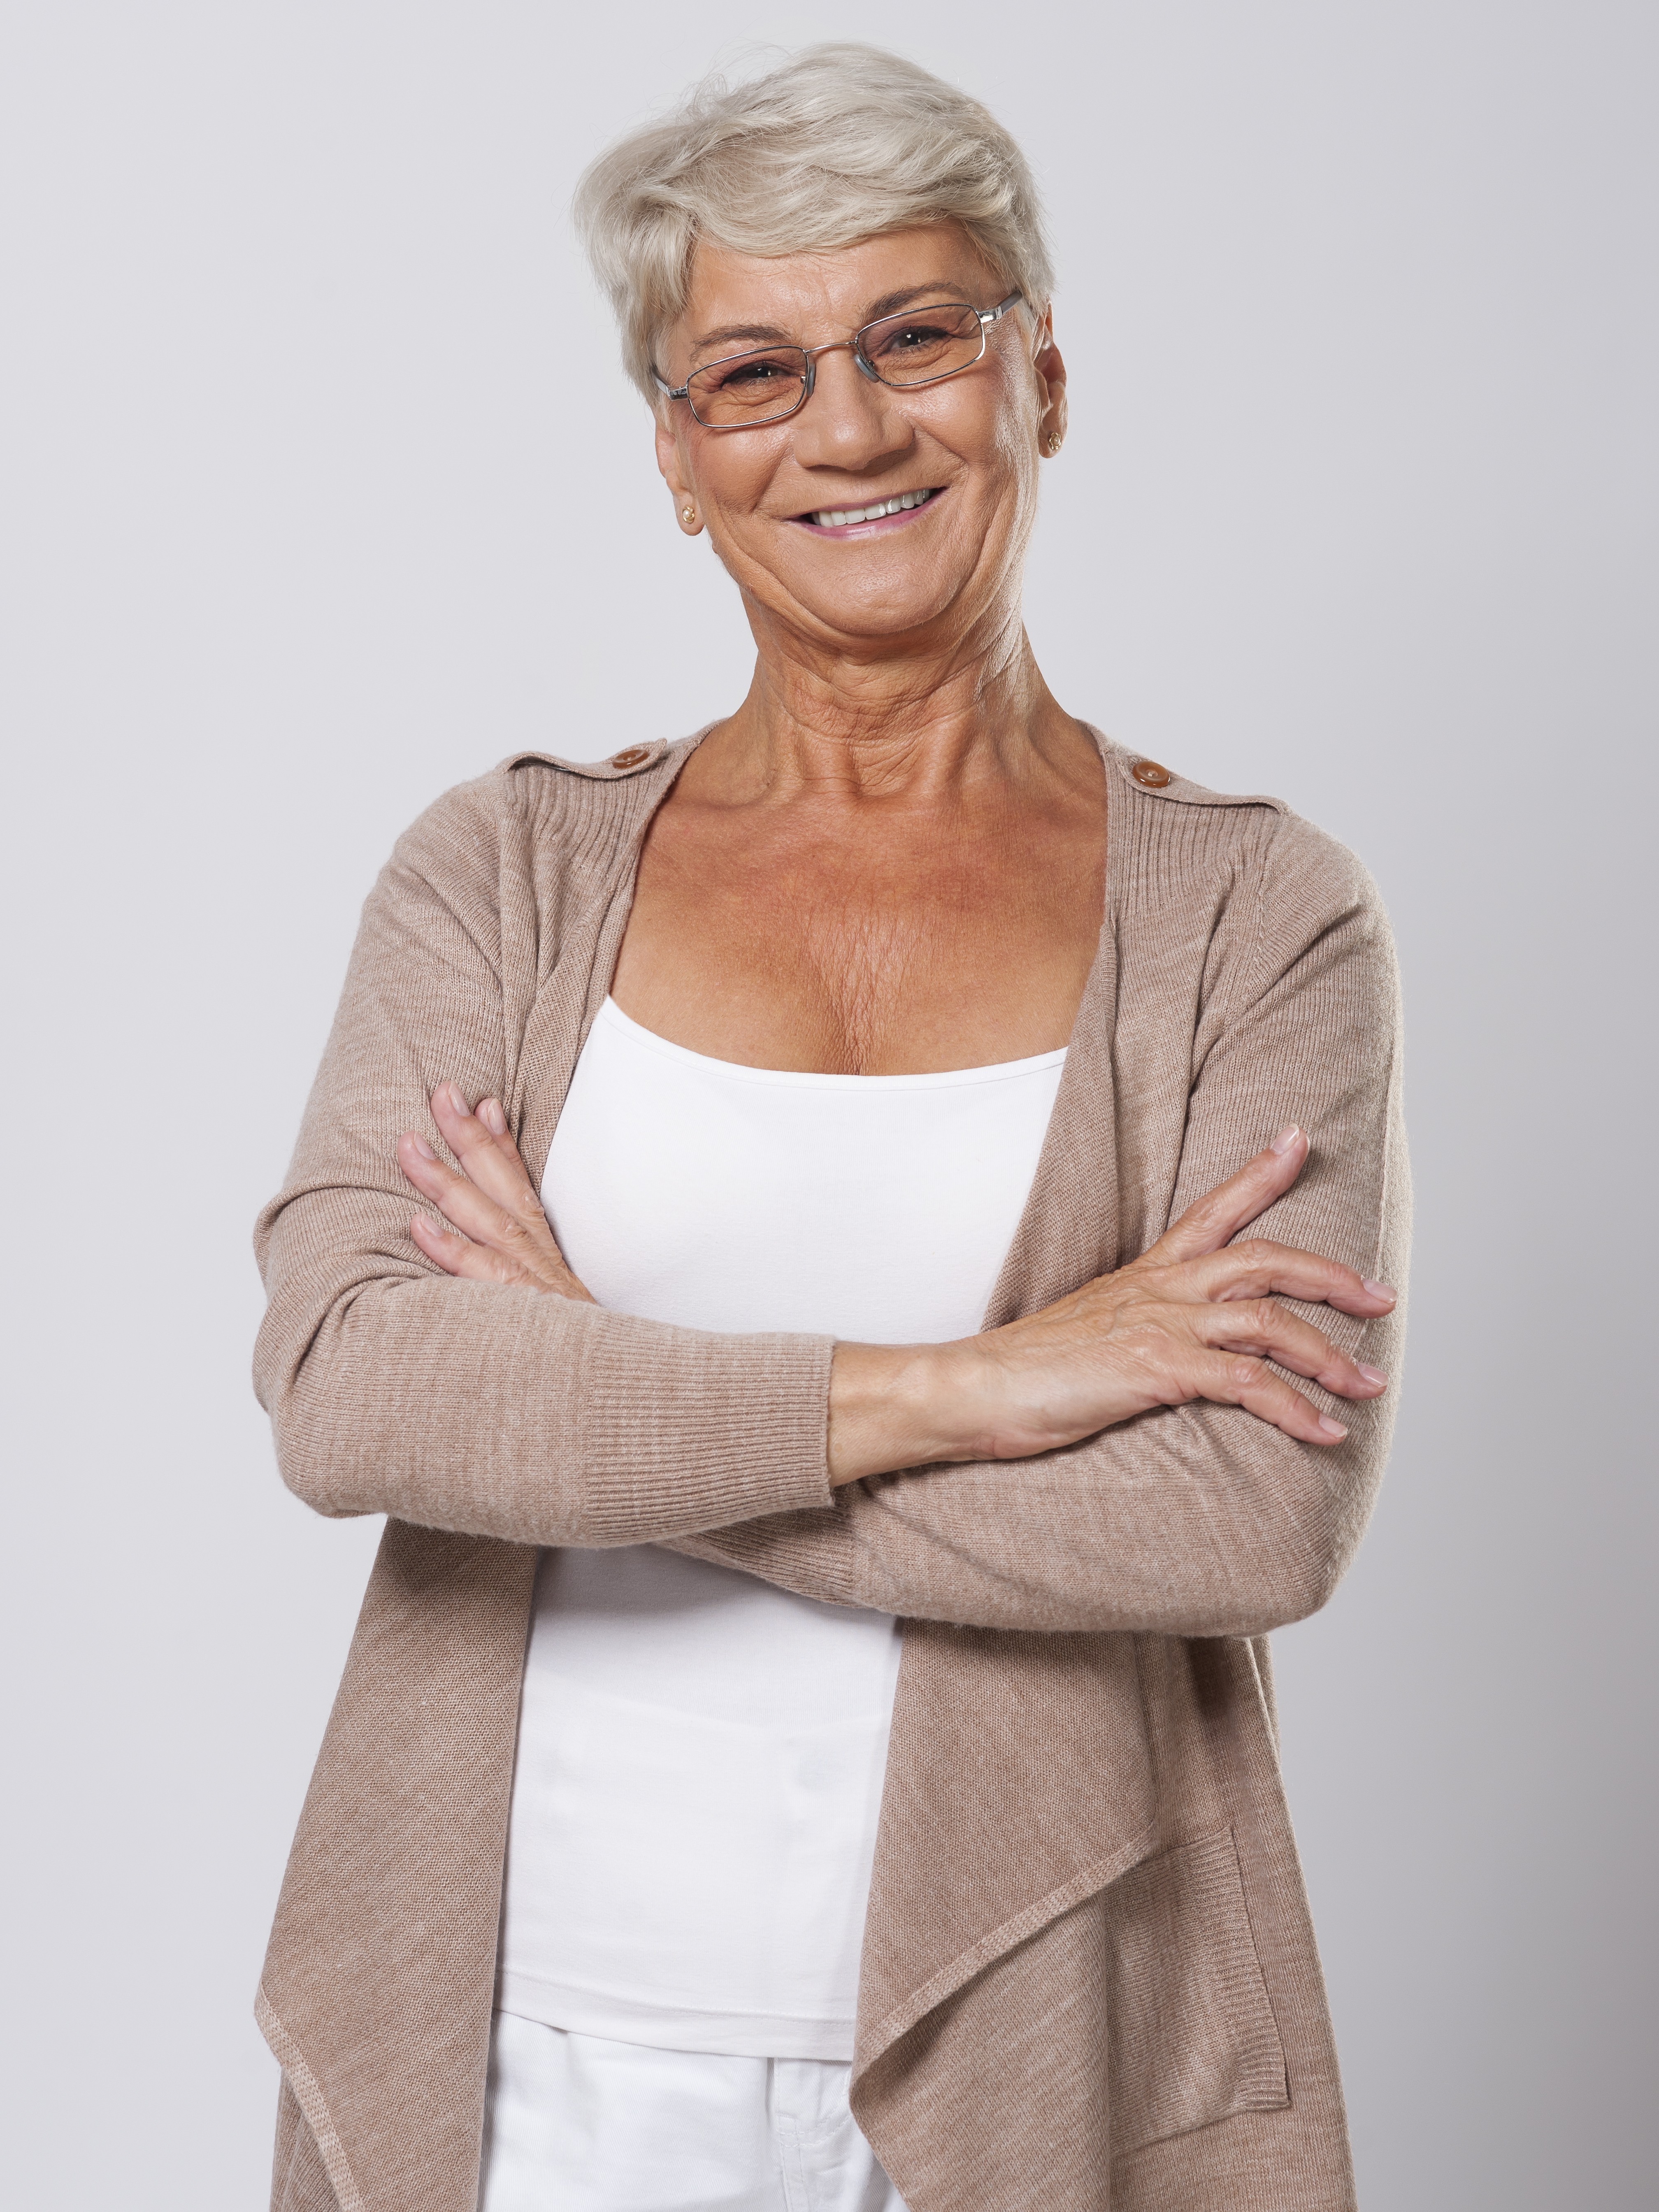
\includegraphics[width=\textwidth]{senhora.jpg}
\end{minipage}%
\hfill
\begin{minipage}{0.6\textwidth}
    \begin{itemize}
        \item \textbf{Nome:} Marlene da Silva (Dona Marlene)
        \item \textbf{Idade:} 58 anos
        \item \textbf{Sexo:} Feminino
        \item \textbf{Estado Civil:} Viúva
        \item \textbf{Ocupação/Trabalho:} Aposentada; cuida informalmente dos netos e sobrinhos-netos enquanto os pais trabalham
        \item \textbf{Biografia:} Funciona como uma espécie de ``creche familiar'', recebendo em casa até 5 crianças com idades entre 6 e 14 anos em horários distintos, contando com um único computador e um tablet compartilhados.
    \end{itemize}
\end{minipage}

\begin{itemize}
    \item \textbf{Hobbies:} Tricô, culinária e cuidar das plantas.
    \item \textbf{Conhecimento em tecnologia:} Baixo.
    \item \textbf{Conhecimento no domínio do negócio:} Médio.
    \item \textbf{Dispositivos que mais utiliza:} Computador de mesa compartilhado.
    \item \textbf{Objetivos dentro do sistema:} Um sistema que funcione no ``piloto automático'', sem exigir troca de perfil a cada criança, garantindo proteção consistente sem configurações complexas.
    \item \textbf{Motivos para utilizar o sistema:} Necessidade de proteção automática em dispositivos compartilhados por crianças de diferentes faixas etárias, sem exigir conhecimentos técnicos avançados de sua parte.
\end{itemize}


\section{Persona 3 -- Caio ``Modo Anônimo'', o Adversário}

\noindent
\hspace{0.7cm}%
\begin{minipage}{0.38\textwidth}
    \centering
    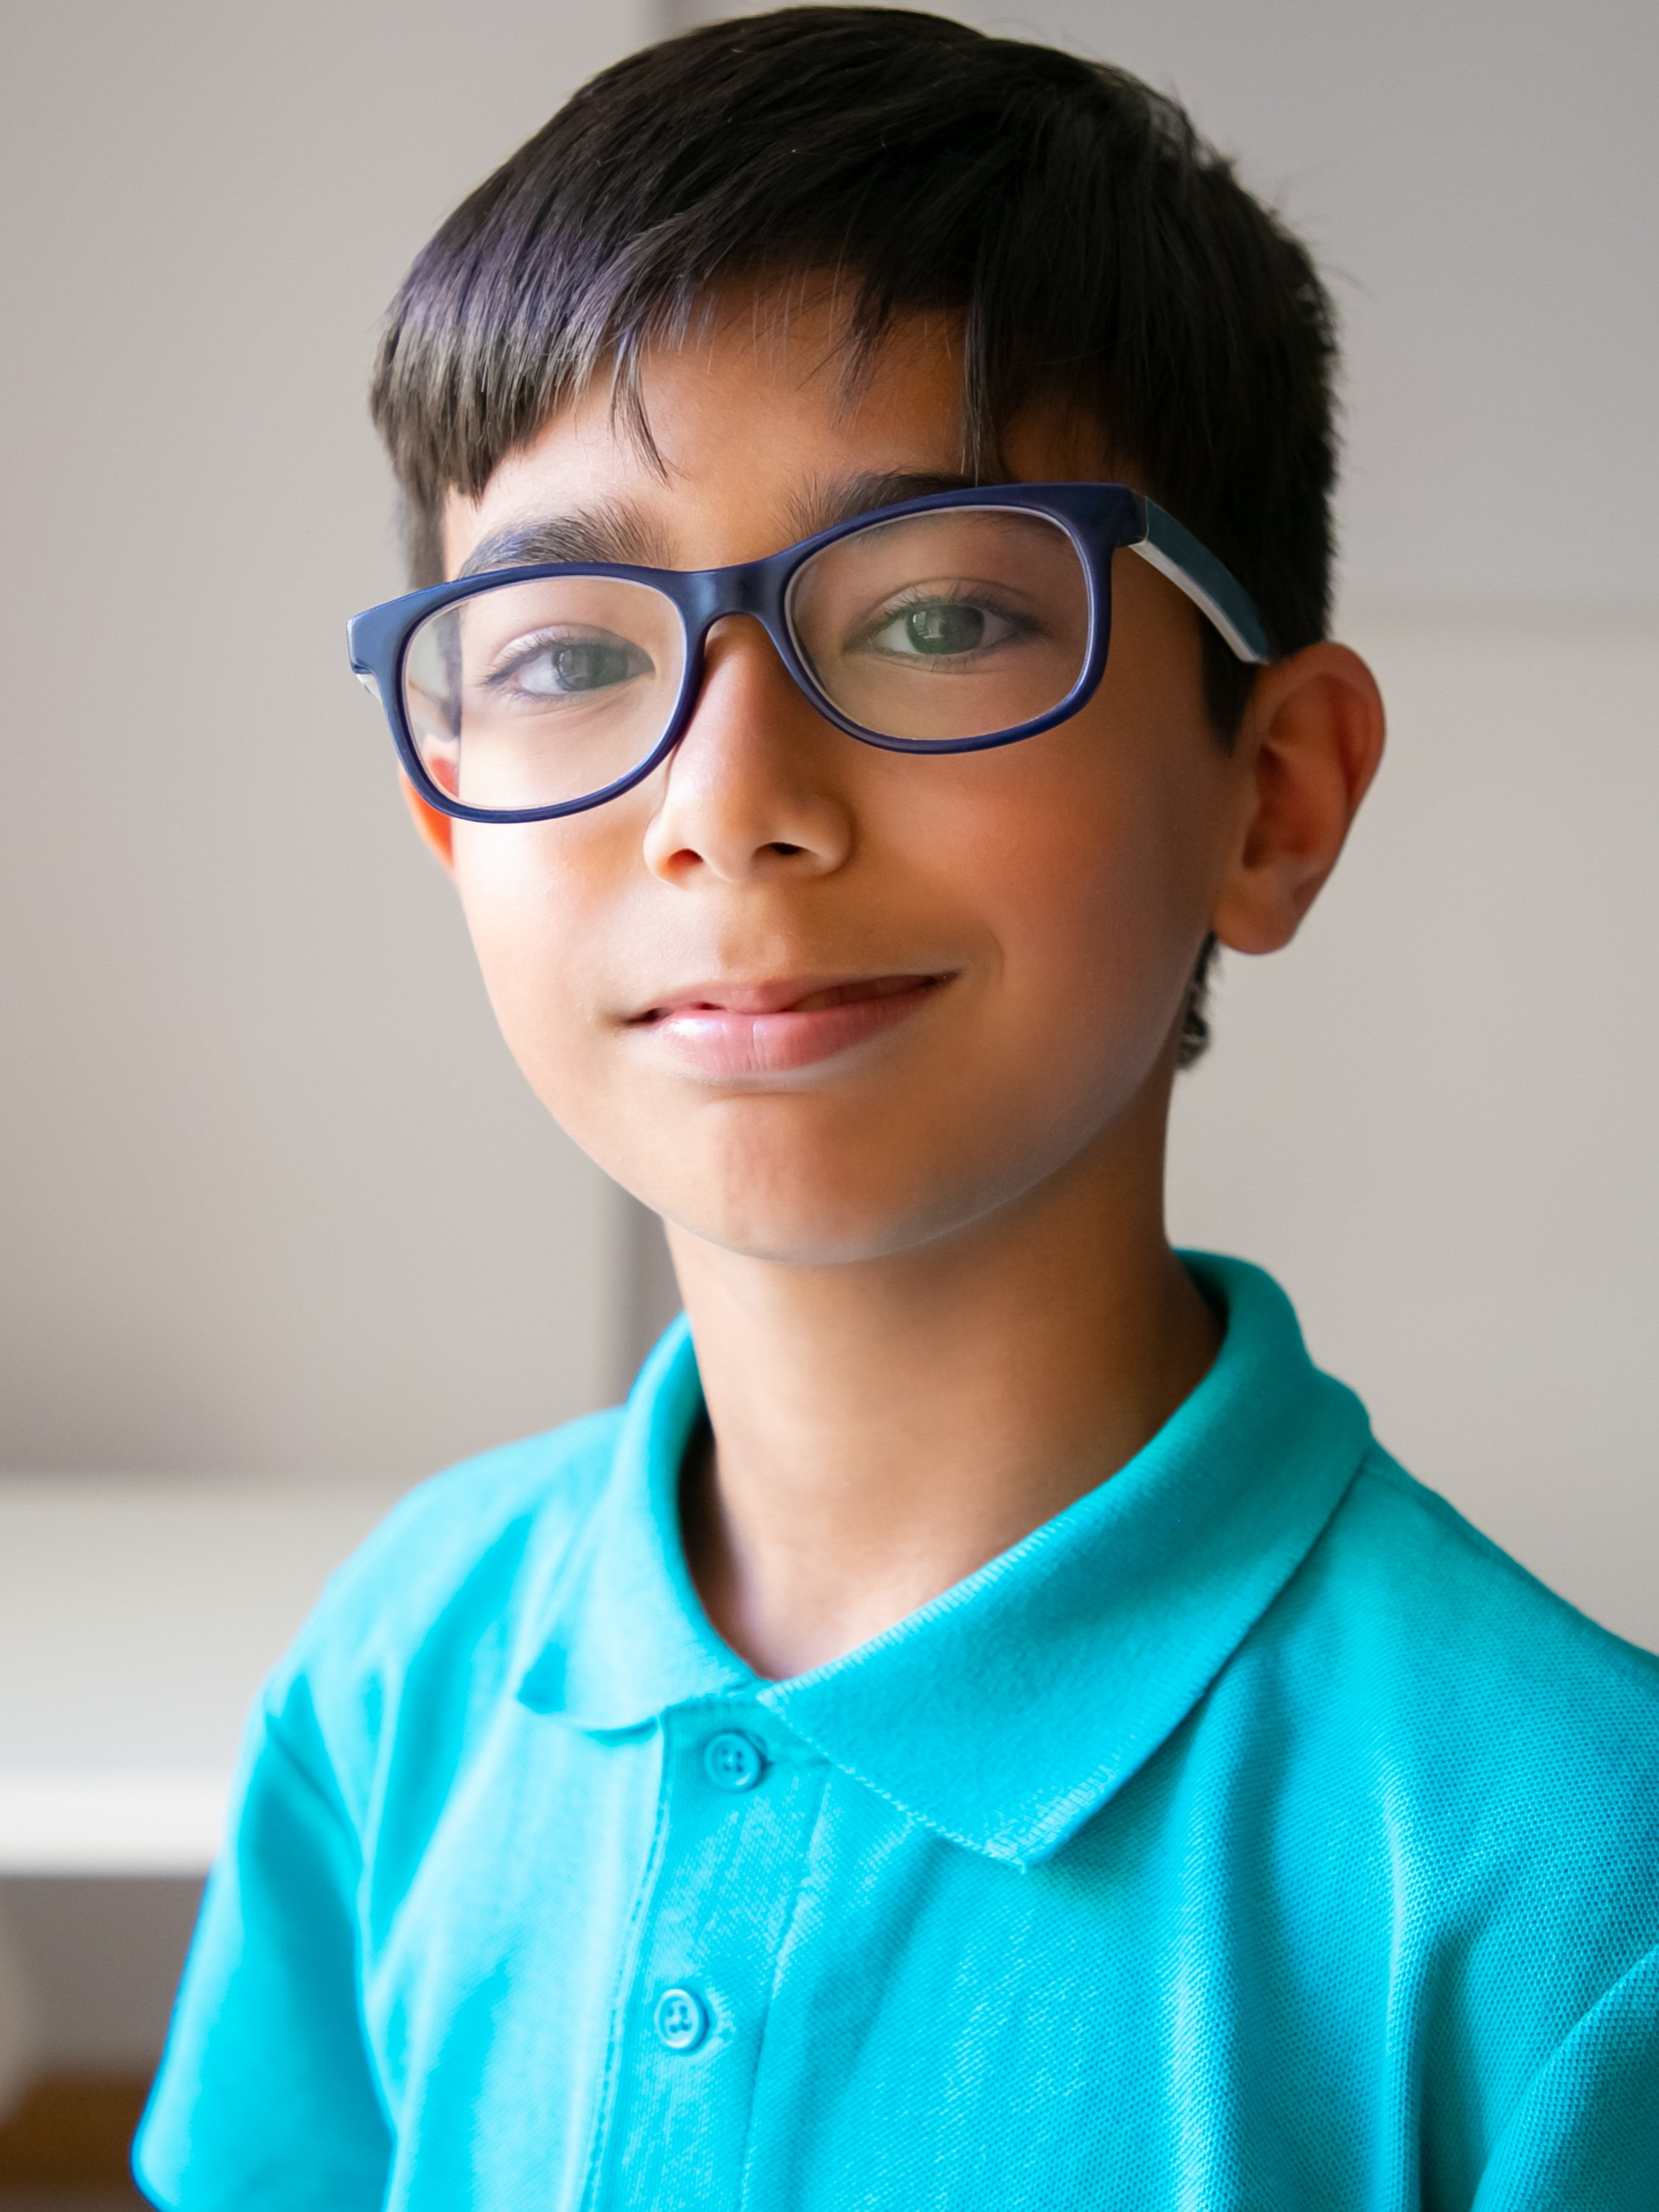
\includegraphics[width=\textwidth]{menino.jpg}
\end{minipage}%
\hfill
\begin{minipage}{0.6\textwidth}
    \begin{itemize}
        \item \textbf{Nome:} Caio Mendes
        \item \textbf{Idade:} 13 anos
        \item \textbf{Sexo:} Masculino
        \item \textbf{Estado Civil:} Solteiro (Estudante)
        \item \textbf{Ocupação/Trabalho:} Estudante do 8º ano
        \item \textbf{Biografia:} Autoproclamado ``especialista em TI'' da família. Usa o tablet da casa compartilhado com os pais e irmão mais novo; já alterou configurações de rede por curiosidade para testar limites.
    \end{itemize}
\end{minipage}

\begin{itemize}
    \item \textbf{Hobbies:} Jogos eletrônicos, vídeos de tecnologia e exploração de softwares.
    \item \textbf{Conhecimento em tecnologia:} Alto para a idade.
    \item \textbf{Conhecimento no domínio do negócio:} Baixo.
    \item \textbf{Dispositivos que mais utiliza:} Tablet e smartphone.
    \item \textbf{Objetivos dentro do sistema:} Acessar conteúdo sem restrição por curiosidade ou para testar os limites do sistema, entendendo como a ferramenta decide o que bloquear.
    \item \textbf{Motivos para testar o sistema:} Representa o caso de uso adversarial essencial para validar os requisitos de segurança, integridade de registros e robustez da arquitetura de IA.
\end{itemize}


% ------------------------------------------------------------
% 8 Protótipos das Interfaces
% ------------------------------------------------------------
\chapter{Protótipos das Interfaces}

Print, legível, das interfaces, no arquivo do relatório final .docx e também o link do
software utilizado para o design (ex: link do figma, XD etc.).

Não será aceito apenas o link.

Validação/aceite dos protótipos com as pessoas/profissionais da comunidade externa.

% ------------------------------------------------------------
% 9 {Modelo de Dados 
% ------------------------------------------------------------
\chapter{Modelo de Dados}

MER para banco de dados relacional ou modelo da estrutura de dados para banco de dados
não relacional.


% ------------------------------------------------------------
% 10 Arquitetura e Tecnologias 
% ------------------------------------------------------------
\chapter{Arquitetura e Tecnologias}

Descrever a arquitetura geral do sistema, incluindo o diagrama/modelo arquitetural e a
integração dos componentes de IA e/ou demais tecnologias atuais do projeto.

Descrever as tecnologias, linguagens, frameworks e bibliotecas utilizadas no
desenvolvimento do sistema (frontend, protótipos, backend, banco de dados, cloud etc).

% ------------------------------------------------------------
% 11 Descrição da Solução de Inteligência Artificial ou outra Tecnologia Atual do Projeto
% ------------------------------------------------------------
\chapter{Descrição da Solução Tecnologica Atual do Projeto}

\section{Base de Dados}

\section*{Processamento de Linguagem Natural (PLN)}
O projeto PI6-ORCA utiliza uma base de dados textual para o desenvolvimento de um modelo
de Inteligência Artificial capaz de classificar textos em três categorias: seguro, suicídio
e ódio. A solução combina dados de duas fontes principais: o conjunto Boamente e o conjunto TuPyE.

Os dados são consolidados e organizados por meio do pipeline de preparação de dados do projeto.
Durante esse processo, os rótulos originais são convertidos para as três classes utilizadas pelo
classificador, permitindo que as diferentes fontes sejam integradas em uma estrutura comum.

Após a preparação inicial, os dados são divididos em três conjuntos: treinamento, validação e
teste, utilizando a proporção de 70%, 15% e 15%, respectivamente, com estratificação por classe e fonte dos dados.

A divisão inicial registrada contém 40.178 textos, distribuídos da seguinte forma:
\begin{itemize}
    \item Treinamento: 28.124 textos.
    \item Validação: 6.027 textos.
    \item Teste: 6.027 textos.
\end{itemize}

Durante a execução do treinamento, são aplicadas verificações adicionais para evitar que textos
iguais ou equivalentes, após a normalização, apareçam em diferentes conjuntos. Com isso, o
treinamento oficial utilizou efetivamente 28.090 textos, enquanto a validação utilizou 6.025 textos.
O conjunto de teste permaneceu com 6.027 textos.

A base apresenta um desequilíbrio na quantidade de exemplos por classe, com predominância da
categoria “seguro” e menor quantidade de exemplos da categoria “suicídio”. Para reduzir o impacto
desse desequilíbrio durante o aprendizado, o treinamento utiliza pesos de classe calculados a partir
da frequência de cada categoria.

\section{Pré-processamento dos Dados}

\section*{Processamento de Linguagem Natural (PLN)}
O pré-processamento tem como objetivo padronizar os textos, reduzir inconsistências e evitar que
informações repetidas entre os conjuntos comprometam a avaliação do modelo.

A normalização utilizada, identificada como norm-v1, aplica as seguintes operações:
\begin{itemize}
    \item Normalização Unicode no formato NFC.
    \item Remoção de links iniciados por http://, https:// ou www..
    \item Remoção do marcador @user, sem distinção entre letras maiúsculas e minúsculas.
    \item Substituição de sequências de espaços e quebras de linha por espaços padronizados.
    \item Remoção de espaços no início e no final dos textos.
    \item Preservação de letras maiúsculas e minúsculas, pois o modelo utilizado diferencia essas características.
\end{itemize}

Além da normalização, o pipeline verifica textos vazios, duplicidades e divergências de classificação.
Quando um mesmo texto normalizado aparece em conjuntos diferentes, são aplicadas regras para evitar
vazamento de dados entre treinamento, validação e teste.

O conjunto de teste permanece inalterado e é utilizado apenas para detectar possíveis colisões durante
essa verificação. As linhas removidas dos conjuntos de treinamento e validação são registradas em um
arquivo específico de auditoria, sem modificar os arquivos CSV originais.

Os textos são tokenizados de acordo com o tokenizador associado ao modelo BERTimbau Base. O comprimento
máximo configurado é de 128 tokens por sequência. Textos que ultrapassam esse limite são truncados,
conforme a configuração do treinamento.

\section{Modelos de IA Utilizados}

\section*{Processamento de Linguagem Natural (PLN)}
O projeto utiliza o modelo pré-treinado BERTimbau Base, disponibilizado pelo identificador
neuralmind/bert-base-portuguese-cased. Trata-se de um modelo baseado na arquitetura BERT, pré-treinado
em português brasileiro e adaptado, por meio de fine-tuning, para a tarefa de classificação de textos.

O modelo foi escolhido por ser adequado ao processamento de textos em português, ser compatível com
as bibliotecas utilizadas no projeto e apresentar um custo computacional mais viável do que a versão
Large para a execução em CPU.

A camada de classificação é configurada para produzir uma das três categorias definidas pelo projeto:
\begin{itemize}
    \item seguro;
    \item suicidio;
    \item odio.
\end{itemize}

O treinamento é realizado com PyTorch e Transformers. A configuração oficial, identificada como nlp-v1,
utiliza os seguintes parâmetros:

\begin{table}[!htbp]
\centering
\small
\renewcommand{\arraystretch}{1.4}
\begin{tabular}{|l|l|}
\hline
\textbf{Parâmetros} & \textbf{Configuração} \\
\hline
Modelo base & BERTimbau Base \\
\hline
Comprimento máximo & 128 tokens \\
\hline
Número de épocas & 3 \\
\hline
Batch size de treinamento & 16 \\
\hline
Batch size de avaliação & 32 \\
\hline
Taxa de aprendizado & 0,00002 \\
\hline
Otimizador & AdamW (adamw\_torch) \\
\hline
Weight decay & 0,01 \\
\hline
Warmup ratio & 0,1 \\
\hline
Agendador da taxa de aprendizado & Linear \\
\hline
Limite de norma do gradiente & 1,0 \\
\hline
Semente aleatória & 42 \\
\hline
Precisão mista FP16/BF16 & Desativada \\
\hline
Ponderação das classes & Inversa da frequência \\
\hline
\end{tabular}
\caption{Exemplo de dados do projeto}
\label{tab:exemplo}
\end{table}

\vspace{2cm}

Os pesos das classes são calculados pela fórmula:

\[
\mathbf{Peso\ da\ classe} = \frac{N}{K \times n^c}
\]

Nessa expressão, $N$ representa o número total de exemplos utilizados no treinamento, $K$ representa
a quantidade de classes e $n^c$ representa a quantidade de exemplos da classe considerada. Essa
estratégia aumenta a contribuição das classes menos frequentes para a função de perda.


\section{Treinamento e Validação}

\section*{Processamento de Linguagem Natural (PLN)}
O treinamento consiste no ajuste dos parâmetros do BERTimbau Base para a classificação dos textos nas
três categorias definidas. Durante esse processo, o modelo aprende padrões linguísticos presentes nos
exemplos rotulados, utilizando a função de perda ponderada para considerar o desequilíbrio entre as
classes.

O treinamento oficial registrado foi executado em CPU durante três épocas, totalizando 5.268 passos.
A configuração efetivamente utilizada corresponde à configuração definida no arquivo nlp-v1.json, sem
diferenças registradas entre os parâmetros configurados e os parâmetros efetivos.

Ao final de cada época, o desempenho é avaliado no conjunto de validação. A seleção do melhor checkpoint
utiliza a métrica Macro F1, que calcula a média do F1-score das classes, atribuindo a mesma importância
a cada uma delas. Dessa forma, a seleção não depende exclusivamente do desempenho na classe majoritária.

O melhor resultado de validação foi registrado na terceira época, no checkpoint checkpoint-5268, com
Macro F1 de aproximadamente 0,7995. Esse checkpoint foi reavaliado, e as métricas registradas foram
consistentes com as métricas utilizadas na seleção.

Além do treinamento oficial, foi realizado um teste rápido identificado como nlp-v1-teste. Essa execução
utilizou uma amostra reduzida de 192 textos para treinamento, 96 para validação e apenas uma época. Seu
objetivo foi verificar o funcionamento do fluxo de treinamento, não substituir a avaliação do modelo
oficial.

O conjunto de teste possui 6.027 textos. Entretanto, os metadados disponibilizados registram as métricas
de validação do modelo oficial, não os resultados de uma avaliação final nesse conjunto de teste.
Portanto, o desempenho no teste independente deve ser documentado após a execução e o registro dessa
avaliação.

\section{Métricas de Avaliação}

\section*{Processamento de Linguagem Natural (PLN)}
A avaliação do classificador utiliza métricas que permitem analisar tanto o desempenho geral quanto a
capacidade de identificar cada uma das três categorias.

As principais métricas adotadas são:
\begin{itemize}
    \item \textbf{Acurácia}: proporção de previsões corretas em relação ao total de exemplos avaliados.
    \item \textbf{Precisão}: proporção de previsões de determinada classe que realmente pertencem a essa classe.
    \item \textbf{Recall}: proporção de exemplos reais de determinada classe que foram identificados corretamente.
    \item \textbf{F1-score}: média harmônica entre precisão e revocação, permitindo avaliar o equilíbrio entre essas duas métricas.
    \item \textbf{Macro F1}: média dos F1-scores das classes, atribuindo o mesmo peso a cada categoria.
    \item \textbf{Matriz de confusão}: tabela que compara as classes reais com as classes previstas pelo modelo, permitindo observar acertos e confusões entre categorias.
\end{itemize}

Na avaliação oficial de validação, o modelo apresentou os seguintes resultados:
\begin{table}[!htbp]
\centering
\small
\renewcommand{\arraystretch}{1.4}
\begin{tabular}{|l|l|}
\hline
\textbf{Métrica} & \textbf{Resultado} \\
\hline
Acurácia & 89,56\% \\
\hline
Macro F1 & 79,95\% \\
\hline
F1-score - seguro & 93,83\% \\
\hline
F1-score - suicídio & 82,11\% \\
\hline
F1-score — ódio & 63,92\% \\
\hline
\end{tabular}
\caption{Resultados da avaliação do modelo no conjunto de validação}
\label{tab:resultados-validacao}
\end{table}

\vspace{4cm}

Os resultados indicam um desempenho elevado na identificação de textos classificados como “seguro” e um F1-score
de 82,11\% para a classe “suicídio”. A classe “ódio” apresentou o menor F1-score, de 63,92\%, indicando maior
dificuldade de classificação nessa categoria.

A matriz de confusão da validação também permite observar que parte dos textos reais da classe “ódio” foi
classificada como “seguro”. Esse comportamento evidencia a necessidade de acompanhar o desempenho individual
das classes, em vez de considerar apenas a acurácia geral.

Os resultados apresentados nesta seção correspondem exclusivamente à validação do modelo oficial nlp-v1. O
resultado do teste rápido, com Macro F1 de aproximadamente 32,41\%, não é utilizado como medida final de
desempenho, pois foi obtido com uma amostra reduzida e somente uma época de treinamento.

A avaliação final no conjunto de teste permanece como uma etapa necessária para verificar a capacidade de
generalização do modelo em dados que não foram utilizados no treinamento nem na seleção do checkpoint.


% ------------------------------------------------------------
% 12 Testes e Validação do Sistema 
% ------------------------------------------------------------
\chapter{Testes e Validação do Sistema}

Apresentar a estratégia de testes de software e os resultados obtidos.

% ------------------------------------------------------------
% 12 Gestão do Projeto 
% ------------------------------------------------------------
\chapter{Gestão do Projeto}

Descrever a metodologia de desenvolvimento adotada (SCRUM), listar o Product Backlog,
cronograma planejado inicial (SPRINTS) com tarefas e responsáveis, cronograma real final
(SPRINTS) com tarefas e responsáveis.

% ------------------------------------------------------------
% 14 Resultados e Discussão 
% ------------------------------------------------------------
\chapter{Resultados e Discussão}

Analisar os resultados obtidos, confrontando-os com os objetivos propostos.

Descrever quais as facilidades e as melhorias que o projeto traz aos usuários, quais os
objetivos foram atendidos e quais objetivos não foram atendidos (e por que não foram
atendidos?).

Fazer as considerações éticas, de privacidade e de impacto social. Discutir possíveis vieses,
impactos sociais, questões éticas e conformidade com legislações de proteção de dados.

% ------------------------------------------------------------
% 15 Conclusão e Trabalhos Futuros 
% ------------------------------------------------------------
\chapter{Conclusão e Trabalhos Futuros}

Apresentar as conclusões do projeto, limitações encontradas e sugestões de melhorias
futuras.

% ------------------------------------------------------------
% 16 Aceite final do projeto 
% ------------------------------------------------------------
\chapter{Aceite final do projeto}

Elaborar um termo de aceite do projeto, pela comunidade externa.

% ------------------------------------------------------------
% REFERÊNCIAS
% ------------------------------------------------------------
\postextual

\chapter{Referências}

\begin{thebibliography}{9}

% APENAS DE EXEMPLO
\bibitem{springbootdocs2026}
SPRING.
Spring Boot Reference Documentation.
\textbf{Spring Framework Docs}, 2026.
Disponível em: \url{https://docs.spring.io/spring-boot/docs/current/reference/html/}.
Acesso em: 10 ago. 2026.

\end{thebibliography}
\end{document}
